\chapter[Estratégias evolutivas para o PRM]{Estratégias evolutivas para o PRM}

A modelagem de um algoritmo genético para o problema do roteamento multicast não é trivial, pois a solução não pode ser representada por um vetor. De fato, como deve representar os caminho entre o servidor e os múltiplos destinos em uma rede de computadores, a solução para o PRM é uma árvore. Dessa forma, é preciso desenvolver o processo de crossover e de mutação de acordo com a estrutura. O cruzamento deve receber duas árvores e gerar uma nova que compartilha características de ambos os pais, enquanto a mutação precisa criar uma pequena alteração na árvore que permita melhor explorar o espaço de busca, mas que não a descaracterize completamente.

Em contrapartida, o PRM se aproxima da definição original do ACO, pois trabalha com grafos. A diferença está no fato de que a solução é representada por uma árvore ao invés de um simples caminho, fazendo com que o depósito de feromônio e a escolha de arestas sejam desenvolvidas conforme a nova estrutura.

\section{Representação da solução}

Como mostrado na seção [seção do prm], considerando que em cada nó da rede a mensagem pode ser replicada e enviada aos próximos nós conectados, o PRM deseja encontrar a árvore que representa o processo de transmissão de menor custo que parte do nó fonte (servidor) e atinge todos os destinos. Existem duas maneiras de se representar a solução:

\begin{enumerate}
	\item Representação em árvore: o AG evolui a própria árvore que se deseja encontrar como solução. É um processo mais complicado que a alternativa a seguir, mas nenhum pós-processamento é necessário.
	\item Representação em conjunto: o AG evolui um conjunto de caminhos $C$, ou seja, para cada nó destino $d$ no problema deve existir uma lista de nós $L \in C$ que contém a sequência de nós, onde o primeiro elemento é o servidor e o último é $d$. A representação em conjuntos é mais fácil de se gerenciar, mas exige a transformação em árvore ao final do processo. Como diferentes árvores podem ser formadas a partir de um conjunto de caminhos, essa representação não é tão eficiente quanto a anterior ao explorar o espaço de busca.
\end{enumerate}

Neste trabalho optou-se por utilizar a representação 1, árvores.

\section{Inicialização dos indivíduos}

\section{Cruzamento (AG)}

O modelo de cruzamento para o PRM utilizado neste trabalho é chamado de cruzamento por caminho e foi proposto em [dissertacao do Fialho] como uma alternativa ao cruzamento por similaridade utilizado em trabalhos anteriores [Bueno e Oliveira, 2010].

O cruzamento por caminho é realizado entre duas árvores $P_1$ e $P_2$ e produz um único filho $F$. O processo consiste em separar cada um dos pais em ramos e então, para cada nó destino $d$ do PRM, acrescentar a $F$ ou o ramo de $P_1$ que leva a $d$, ou o ramo de $P_2$. A escolha entre $P_1$ e $P_2$ é feita de forma aleatória. Assim que todos os nós destinos são atingíveis em $F$, para-se a seleção de ramos, remove-se os ciclos que possivelmente foram incluídos e poda-se a árvore, excluindo qualquer nó folha que não seja um destino.

\begin{figure}[!htbp]
	\label{fig_prm-cruzamento-caminho}
	\caption{Exemplo de cruzamento por caminho}
	\centering
	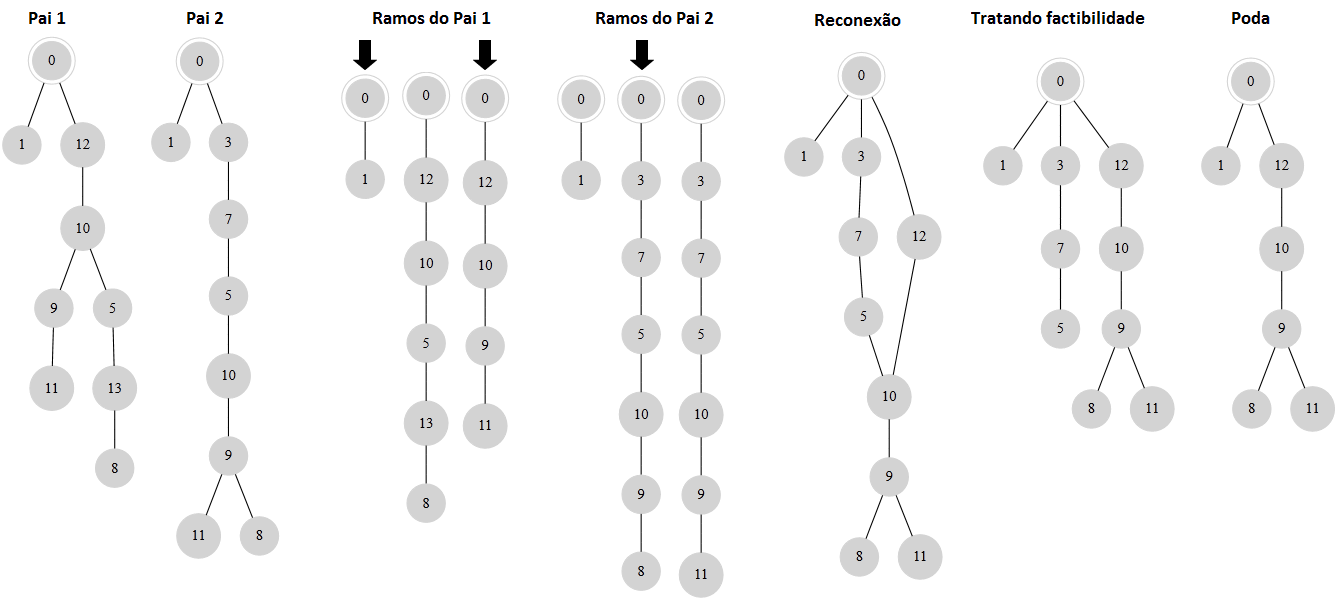
\includegraphics[width=1\textwidth]{cap_estrategias-prm/figs/prm-cruzamento-caminho}
\end{figure}

A figura \ref{fig_prm-cruzamento-caminho}, retirada do trabalho de [dissertacao Fialho], representa o processo de cruzamento por caminho entre duas árvores (Pai 1 e Pai 2). No exemplo, o nó raiz (servidor) é o vértice 0 e os destinos são o conjunto $\{1, 8, 11\}$. As setas em ``ramos do pai 1'' e ``ramos do pai 2'' representam os caminhos escolhidos em cada um dos pais para compor a árvore filha. O grafo nomeado ``reconexão'' representa o filho após a inclusão de todos os ramos, e como foi gerado um ciclo, deve-se removê-lo afim de obter-se uma árvore válida. Em ``tratando factibilidade'' apresenta-se o filho após a remoção dos ciclos, como o nó folha ``5'' não é um destino, deve-se podá-lo, resultando na última árvore, ``poda'', que é o filho retornado pelo processo.

Durante o processo de cruzamento por caminho, para remover os ciclos, percorre-se a árvore em largura removendo qualquer aresta que adicione ciclo. No processo de poda, verifica-se todas as folhas, se alguma não for um destino, remove-se o nó, repetindo o processo até que todos os nós folhas sejam destinos.

\section{Mutação (AG)}

A mutação em uma árvore que representa uma solução para o PRM consiste em remover parte dos nós da árvore e então reconectá-los de maneira aleatória utilizando o grafo correspondente à rede em questão. Veja o algoritmo \ref{alg_prm_mutacao}.

\begin{algorithm}
	\caption{Mutação para uma árvore $(A, G, qte_{arestas}, r, D)$}
	\label{alg_prm_mutacao}
	\begin{algorithmic}[1]
		\State Selecione aleatoriamente $qte_{arestas}$ e remova-as de $A$
		\State Retire de $A$ a componente conexa que contém a raiz e chame-a de $C$
		\State Crie um grafo vazio $M$ para guardar o resultado da mutação
		\State Adicione todas as arestas de $C$ a $M$
		\While{$|D| > 0$}
			\State Selecione aleatoriamente um destino $d \in D$ e remova-o da lista $D$
			\State Remova de $A$ a componente conexa correspondente ao destino $d$ e coloque-a em $C$
			\If{$M$ não possui o vértice $d$}
				\State Tendo $G$ como referência, crie um caminho aleatório $P$ entre $M$ e a componente conexa $C$
				\State Adicione todas as arestas de $P$ a $M$
			\EndIf
			\State Adicione todas as arestas de $C$ a $M$
		\EndWhile
		\State Remova os ciclos em $M$, caso existam
		\State Pode a árvore $M$, removendo todos os nós folhas que não são destinos
		\State \Return $M$
	\end{algorithmic}
\end{algorithm}

No algoritmo \ref{alg_prm_mutacao} recebe-se como parâmetros a árvore a se mutar ($A$), o grafo da rede ($G$), a quantidade de arestas a se remover na mutação ($qte_{arestas}$), o vértice raiz ($r$), e o conjunto de destinos ($D$). Na linha 7, se não existe componente conexa com o vértice $d$, $C$ será um grafo com um único nó ($d$) e nenhuma aresta. Na linha 9, o caminho aleatório é construído nó a nó até se encontrar uma sequência de arestas entre as duas componentes. Ao final, o mesmo pós-processamento do cruzamento por caminho é realizado: remove-se os ciclos e poda-se a árvore.

\section{Construção da solução (ACO)}

